%%%%%%%%%%%%%%
%% Run LaTeX on this file several times to get Table of Contents,
%% cross-references, and citations.

%% If you have font problems, you may edit the w-bookps.sty file
%% to customize the font names to match those on your system.

%% w-bksamp.tex. Current Version: Feb 16, 2012
%%%%%%%%%%%%%%%%%%%%%%%%%%%%%%%%%%%%%%%%%%%%%%%%%%%%%%%%%%%%%%%%
%
%  Sample file for
%  Wiley Book Style, Design No.: SD 001B, 7x10
%  Wiley Book Style, Design No.: SD 004B, 6x9
%
%
%  Prepared by Amy Hendrickson, TeXnology Inc.
%  http://www.texnology.com
%%%%%%%%%%%%%%%%%%%%%%%%%%%%%%%%%%%%%%%%%%%%%%%%%%%%%%%%%%%%%%%%

%%%%%%%%%%%%%
% 7x10
%\documentclass{wileySev}

% 6x9
\documentclass{wileySix}

\usepackage{graphicx}
\usepackage{listings}
\usepackage{float}

\usepackage{color}
 
\definecolor{codegreen}{rgb}{0,0.6,0}
\definecolor{codegray}{rgb}{0.5,0.5,0.5}
\definecolor{codepurple}{rgb}{0.58,0,0.82}
\definecolor{backcolour}{rgb}{0.95,0.95,0.92}
 
\lstdefinestyle{mystyle}{
    backgroundcolor=\color{backcolour},   
    commentstyle=\color{codegreen},
    keywordstyle=\color{magenta},
    numberstyle=\tiny\color{codegray},
    stringstyle=\color{codepurple},
    basicstyle=\footnotesize,
    breakatwhitespace=false,         
    breaklines=true,                 
    captionpos=b,                    
    keepspaces=true,                 
    numbers=left,                    
    numbersep=5pt,                  
    showspaces=false,                
    showstringspaces=false,
    showtabs=false,                  
    tabsize=2,
    language=sh
}
 
\lstset{style=mystyle}

%%%%%%%
%% for times math: However, this package disables bold math (!)
%% \mathbf{x} will still work, but you will not have bold math
%% in section heads or chapter titles. If you don't use math
%% in those environments, mathptmx might be a good choice.

% \usepackage{mathptmx}

% For PostScript text
\usepackage{w-bookps}

%%%%%%%%%%%%%%%%%%%%%%%%%%%%%%%%%%%%%%%%%%%%%%%%%%%%%%%%%%%%%%%%
%% Other packages you might want to use:

% for chapter bibliography made with BibTeX
% \usepackage{chapterbib}

% for multiple indices
% \usepackage{multind}

% for answers to problems
% \usepackage{answers}

%%%%%%%%%%%%%%%%%%%%%%%%%%%%%%
%% Change options here if you want:
%%
%% How many levels of section head would you like numbered?
%% 0= no section numbers, 1= section, 2= subsection, 3= subsubsection
%%==>>
\setcounter{secnumdepth}{3}

%% How many levels of section head would you like to appear in the
%% Table of Contents?
%% 0= chapter titles, 1= section titles, 2= subsection titles, 
%% 3= subsubsection titles.
%%==>>
\setcounter{tocdepth}{2}

%% Cropmarks? good for final page makeup
%% \docropmarks

%%%%%%%%%%%%%%%%%%%%%%%%%%%%%%
%
% DRAFT
%
% Uncomment to get double spacing between lines, current date and time
% printed at bottom of page.
% \draft
% (If you want to keep tables from becoming double spaced also uncomment
% this):
% \renewcommand{\arraystretch}{0.6}
%%%%%%%%%%%%%%%%%%%%%%%%%%%%%%

%%%%%%% Demo of section head containing sample macro:
%% To get a macro to expand correctly in a section head, with upper and
%% lower case math, put the definition and set the box 
%% before \begin{document}, so that when it appears in the 
%% table of contents it will also work:

\newcommand{\VT}[1]{\ensuremath{{V_{T#1}}}}

%% use a box to expand the macro before we put it into the section head:

\newbox\sectsavebox
\setbox\sectsavebox=\hbox{\boldmath\VT{xyz}}

%%%%%%%%%%%%%%%%% End Demo


\begin{document}


\booktitle{Cerdas Menguasai Python}
\subtitle{Dalam 24 Jam}

\authors{Rolly M. Awangga\\
\affil{Informatics Research Center}
%Floyd J. Fowler, Jr.\\
%\affil{University of New Mexico}
}

\offprintinfo{Cerdas Menguasai Python, First Edition}{Rolly M. Awangga}

%% Can use \\ if title, and edition are too wide, ie,
%% \offprintinfo{Survey Methodology,\\ Second Edition}{Robert M. Groves}

%%%%%%%%%%%%%%%%%%%%%%%%%%%%%%
%% 
\halftitlepage

\titlepage


\begin{copyrightpage}{2019}
%Survey Methodology / Robert M. Groves . . . [et al.].
%\       p. cm.---(Wiley series in survey methodology)
%\    ``Wiley-Interscience."
%\    Includes bibliographical references and index.
%\    ISBN 0-471-48348-6 (pbk.)
%\    1. Surveys---Methodology.  2. Social 
%\  sciences---Research---Statistical methods.  I. Groves, Robert M.  II. %
%Series.\\
%
%HA31.2.S873 2007
%001.4'33---dc22                                             2004044064
\end{copyrightpage}

\dedication{`Jika Kamu tidak dapat menahan lelahnya belajar, 
Maka kamu harus sanggup menahan perihnya Kebodohan.'
~Imam Syafi'i~}

\begin{contributors}
\name{Rolly Maulana Awangga,} Informatics Research Center., Politeknik Pos Indonesia, Bandung,
Indonesia



\end{contributors}

\contentsinbrief
\tableofcontents
\listoffigures
\listoftables
\lstlistoflistings


\begin{foreword}
Sepatah kata dari Kaprodi, Kabag Kemahasiswaan dan Mahasiswa
\end{foreword}

\begin{preface}
Buku ini diciptakan bagi yang awam dengan git sekalipun.

\prefaceauthor{R. M. Awangga}
\where{Bandung, Jawa Barat\\
Februari, 2019}
\end{preface}


\begin{acknowledgments}
Terima kasih atas semua masukan dari para mahasiswa agar bisa membuat buku ini 
lebih baik dan lebih mudah dimengerti.

Terima kasih ini juga ditujukan khusus untuk team IRC yang 
telah fokus untuk belajar dan memahami bagaimana buku ini mendampingi proses 
Intership.
\authorinitials{R. M. A.}
\end{acknowledgments}

\begin{acronyms}
\acro{ACGIH}{American Conference of Governmental Industrial Hygienists}
\acro{AEC}{Atomic Energy Commission}
\acro{OSHA}{Occupational Health and Safety Commission}
\acro{SAMA}{Scientific Apparatus Makers Association}
\end{acronyms}

\begin{glossary}
\term{git}Merupakan manajemen sumber kode yang dibuat oleh linus torvald.

\term{bash}Merupakan bahasa sistem operasi berbasiskan *NIX.

\term{linux}Sistem operasi berbasis sumber kode terbuka yang dibuat oleh Linus Torvald
\end{glossary}

\begin{symbols}
\term{A}Amplitude

\term{\hbox{\&}}Propositional logic symbol 

\term{a}Filter Coefficient

\bigskip

\term{\mathcal{B}}Number of Beats
\end{symbols}

\begin{introduction}

%% optional, but if you want to list author:

\introauthor{Rolly Maulana Awangga, S.T., M.T.}
{Informatics Research Center\\
Bandung, Jawa Barat, Indonesia}

Pada era disruptif  \index{disruptif}\index{disruptif!modern} 
saat ini. git merupakan sebuah kebutuhan dalam sebuah organisasi pengembangan perangkat lunak.
Buku ini diharapkan bisa menjadi penghantar para programmer, analis, IT Operation dan Project Manajer.
Dalam melakukan implementasi git pada diri dan organisasinya.

Rumusnya cuman sebagai contoh aja biar keren\cite{awangga2018sampeu}.

\begin{equation}
ABC {\cal DEF} \alpha\beta\Gamma\Delta\sum^{abc}_{def}
\end{equation}

\end{introduction}

%%%%%%%%%%%%%%%%%%Isi Buku_

\chapter{SEJARAH DAN KARAKTERISTIK  PYTHON}
\section{Perintah Navigasi}
Perintah navigasi direktori

\section{Harun Ar-Rasyid}
\subsection{Sejarah}
Python diciptakan oleh Guido van Rossum pertama kali di Scitchting Mathematisch Centrum (CWI) di Belanda pada awal tahun 1990-an. Bahasa python terinspirasi dari bahasa pemrograman ABC. Sampai sekarang, Guido masih menjadi penulis utama untuk python, meskipun bersifat open source sehingga ribuan orang juga berkontribusi dalam mengembangkannya.

Pada 1995, Guido pindah ke CNRI di Virginia Amerika sambil terus mengembangkan Python. Versi terakhir yang dirilis adalah 1.6. Pada tahun 2000, pengembang inti Guido dan Python pindah ke BeOpen.com yang merupakan perusahaan komersial dan membentuk BeOpen PythonLabs. Python 2.0 dirilis oleh BeOpen. Setelah menghapus Python 2.0, Guido dan beberapa anggota tim PythonLabs pindah ke DigitalCreations.

Saat ini pengembangan Python terus dilakukan oleh sekelompok programmer yang dikoordinir oleh Guido dan Python Software Foundation. Python Software Foundation adalah organisasi nirlaba yang dibentuk sebagai pemegang hak cipta intelektual Python sejak versi 2.1 dan dengan demikian mencegah Python dimiliki oleh perusahaan komersial. Saat ini distribusi Python telah mencapai versi 2.7.14 dan versi 3.6.3

Nama Python dipilih oleh Guido sebagai nama bahasa ciptaannya karena kecintaan Guido pada acara televisi Flying Circus Monty Python. Oleh karena itu sering ekspresi khas acara sering muncul dalam korespondensi antara pengguna Python.
\subsection{Instalasi Anaconda}
\begin{enumerate}
    \item Pastikan Bahwa Python telah terinstal dilaptop anda.
    \item Jika anda belum punya anaconda, kalian bisa download di https://www.anaconda.com/distribution/#download-section
    \item Kemudian buka installer yang telah di download barusan
    \item Klik next
    \begin{figure}[!htbp]
        \centering
        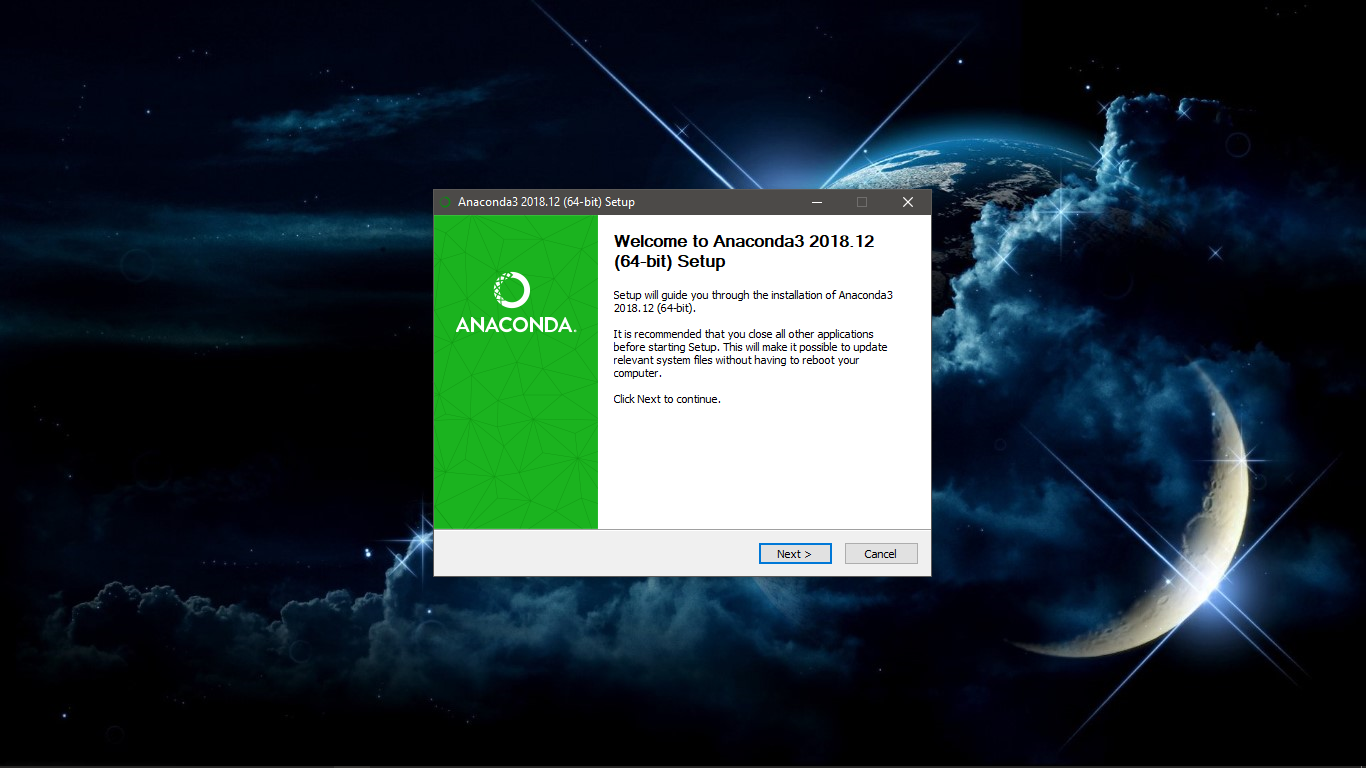
\includegraphics[width=3cm,height=3cm]{figures/Screenshot(80).png}
        \caption{Tampilan Awal}
        \label{awal}
        \end{figure}

    \item Kemudian Klik I Agree
    \begin{figure}[!htbp]
        \centering
        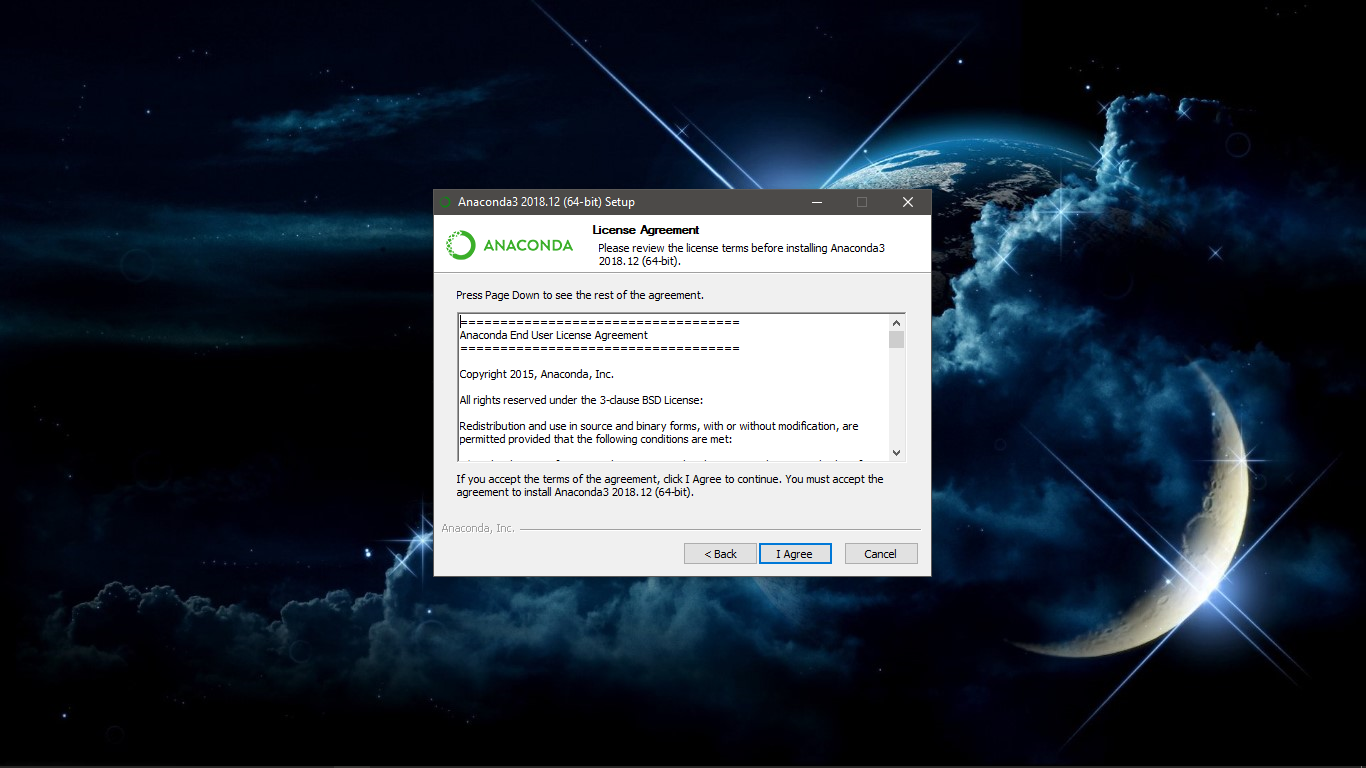
\includegraphics[width=3cm,height=3cm]{figures/Screenshot(81).png}
        \caption{License Agreement}
        \label{License}
        \end{figure}

    \item Kemudian pilih akan di instal untuk siapa, kemudian pilih next
    \begin{figure}[!htbp]
        \centering
        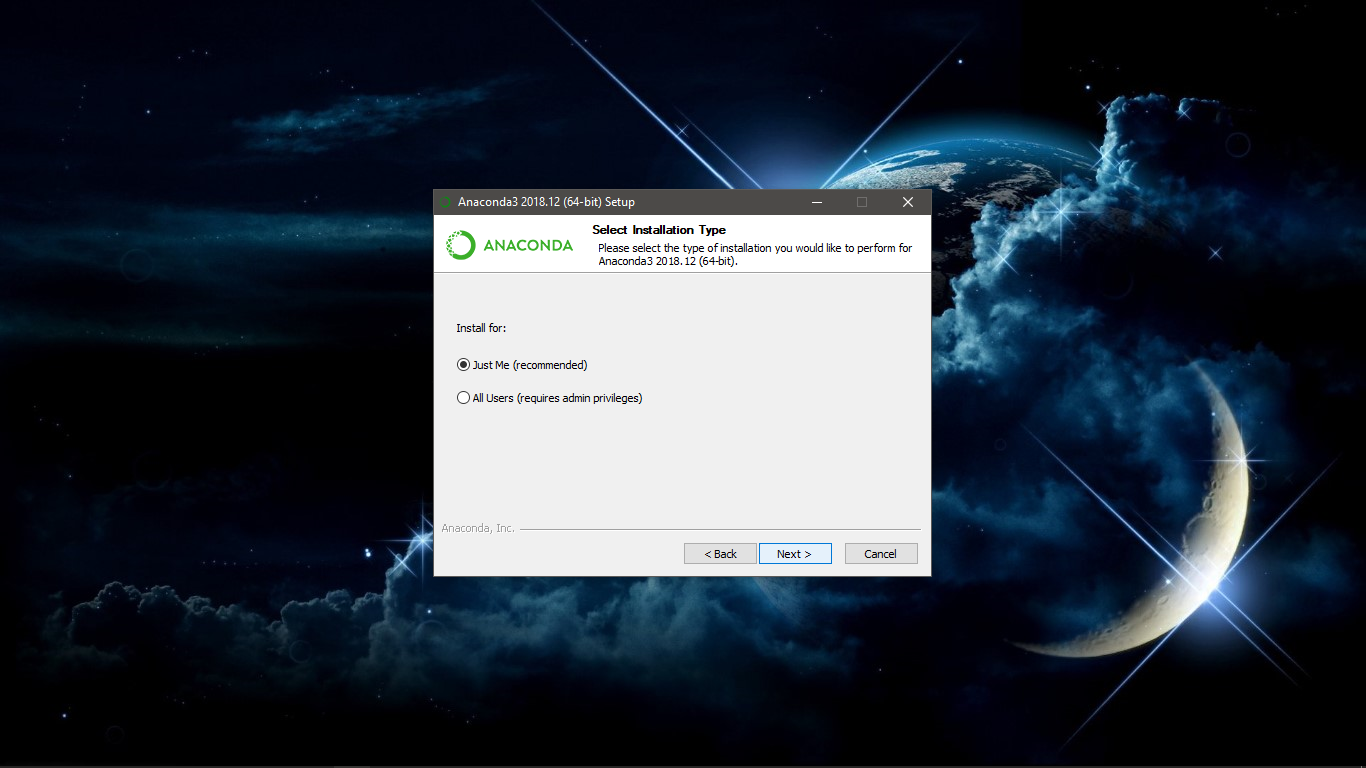
\includegraphics[width=3cm,height=3cm]{figures/Screenshot(82).png}
        \caption{Pemilihan User}
        \label{User}
        \end{figure}

    \item Kemudian tentukan dicretory nya, secara default akan berada di C:\Users\namakomputer\Anaconda3
    \begin{figure}[!htbp]
        \centering
        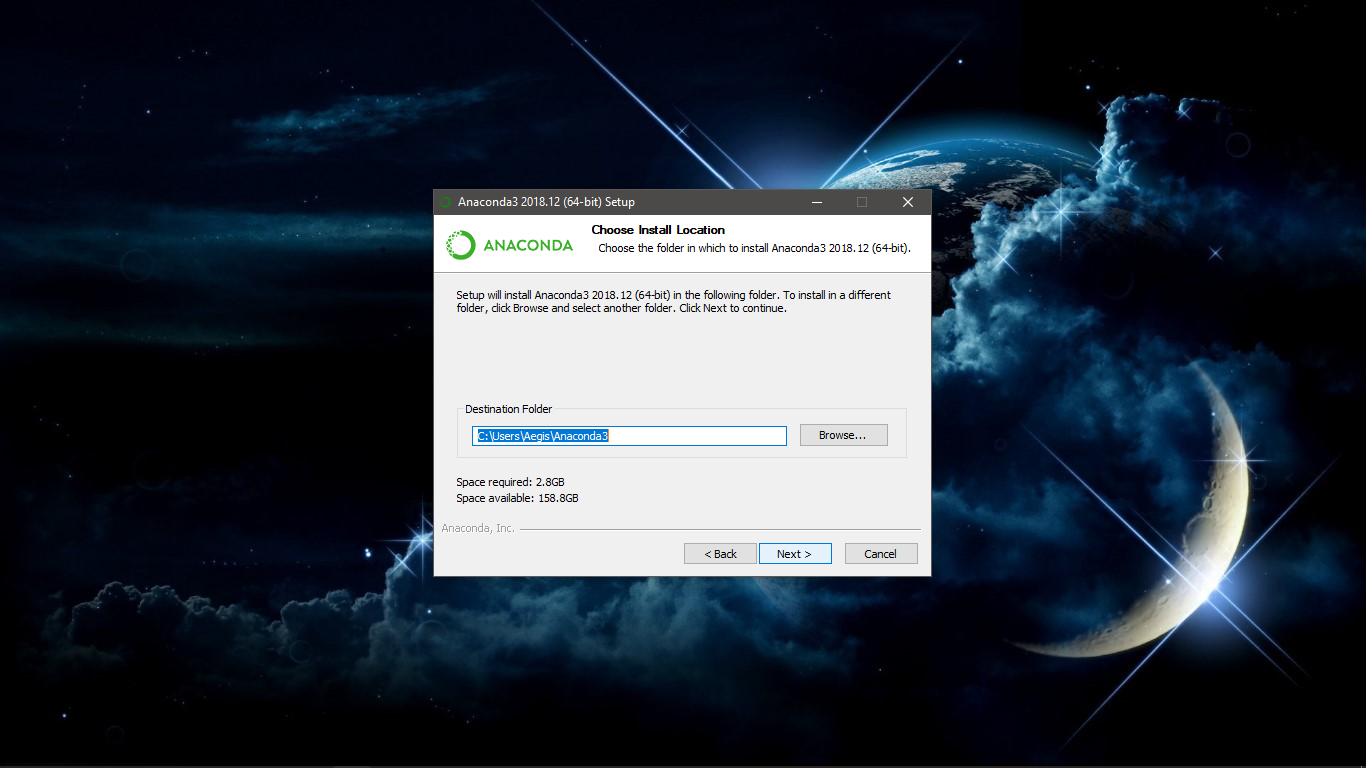
\includegraphics[width=3cm,height=3cm]{figures/Screenshot(83).png}
        \caption{Pemilihan Direktori Penyimpanan}
        \label{Directory}
        \end{figure}

    \item Kemudian Centang yang register Anaconda as default Python, Kemudian Pilih Next
    \begin{figure}[!htbp]
        \centering
        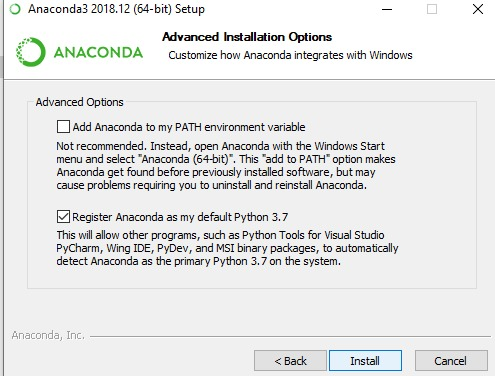
\includegraphics[width=3cm,height=3cm]{figures/Screenshot(84).jpeg}
        \caption{Pemilihan Opsi}
        \label{opsi}
        \end{figure}

    \item Tunggu Proses Instalasi hingga selesai
    \begin{figure}[!htbp]
        \centering
        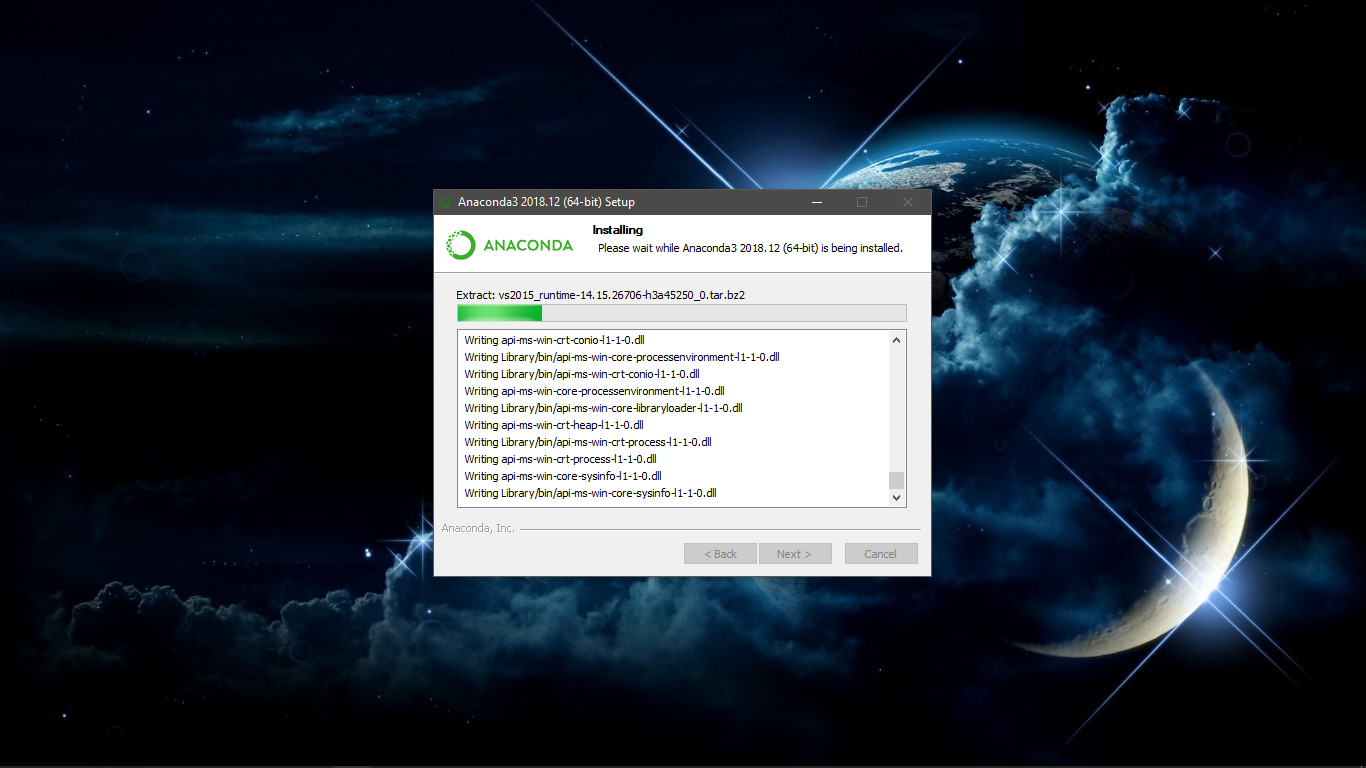
\includegraphics[width=3cm,height=3cm]{figures/Screenshot(85).png}
        \caption{Proses Instal}
        \label{Proses}
        \end{figure}

    \item Klik next
    \begin{figure}[!htbp]
        \centering
        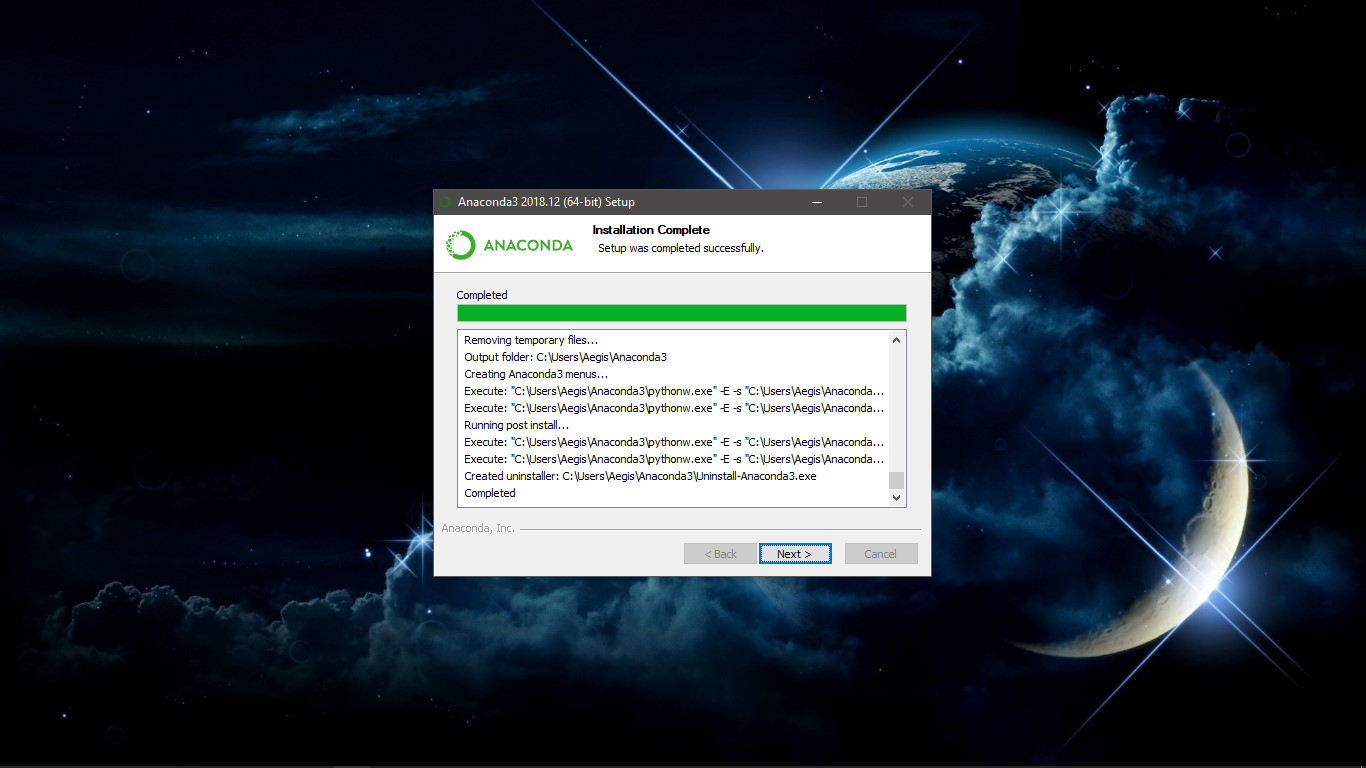
\includegraphics[width=3cm,height=3cm]{figures/Screenshot(86).png}
        \caption{Proses Instal Selesai}
        \label{Proses}
        \end{figure}

    \item kemudian jika kalian belum instal MS VSC di sarankan menginstalnya dlu, jika sudah klik skip
    \begin{figure}[!htbp]
        \centering
        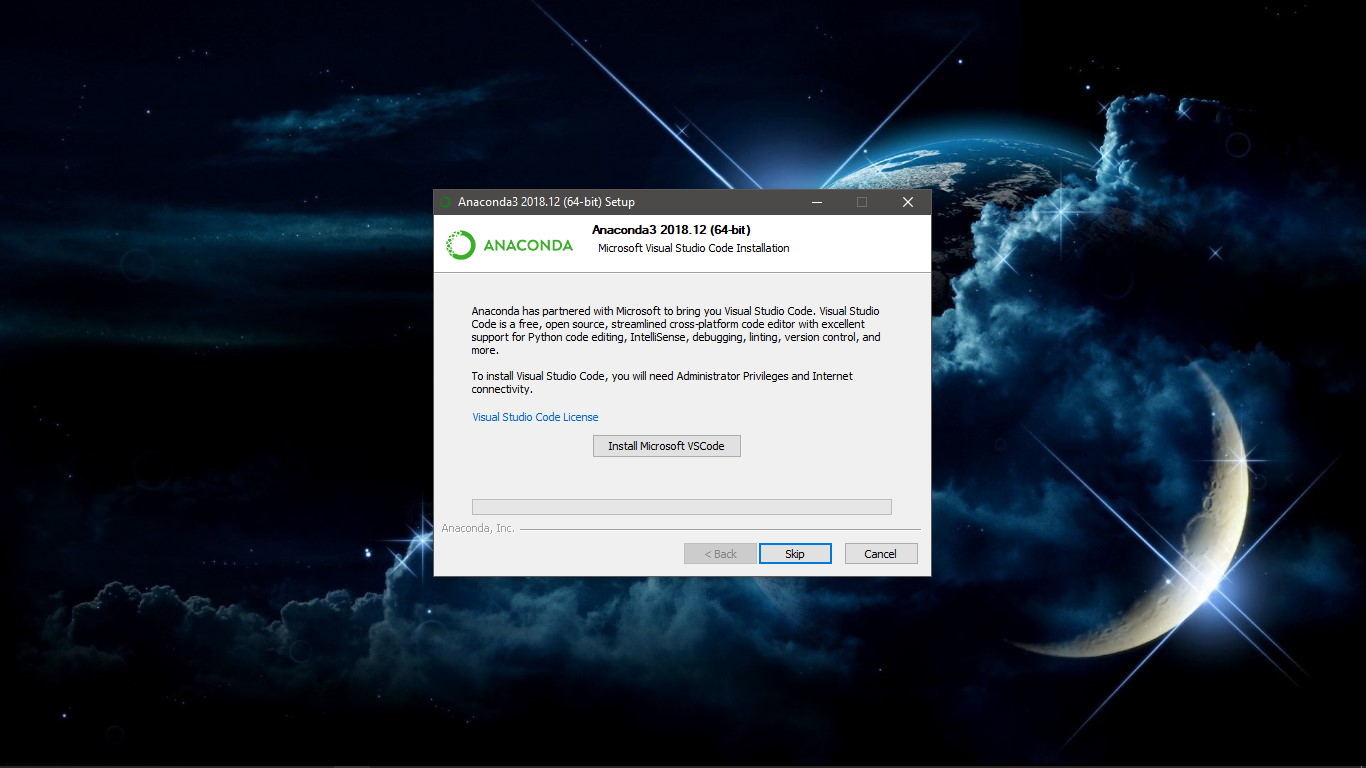
\includegraphics[width=3cm,height=3cm]{figures/Screenshot(87).png}
        \caption{Penawaran Instal MS VSC}
        \label{offering}
        \end{figure}

    \item Instalasi anaconda telah selesai
    \begin{figure}[!htbp]
        \centering
        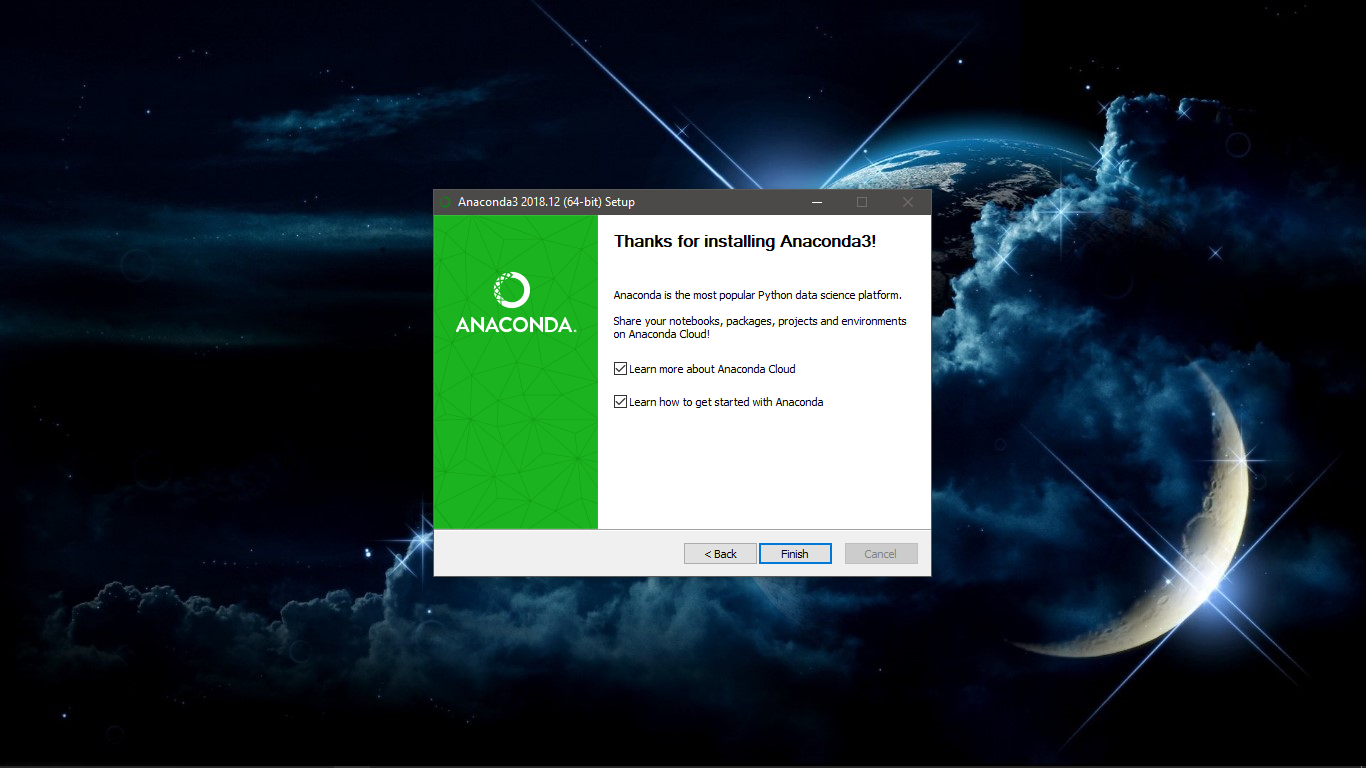
\includegraphics[width=3cm,height=3cm]{figures/Screenshot(88).png}
        \caption{Instalasi Selesai}
        \label{akhir}
        \end{figure}
\end{enumerate}
\subsection{Menggunakan Spyder}
Setelah selesai melakukan instalasi anaconda, maka ada beberapa tool yang digunakan seperti spyder

\begin{figure}[!htbp]
    \centering
    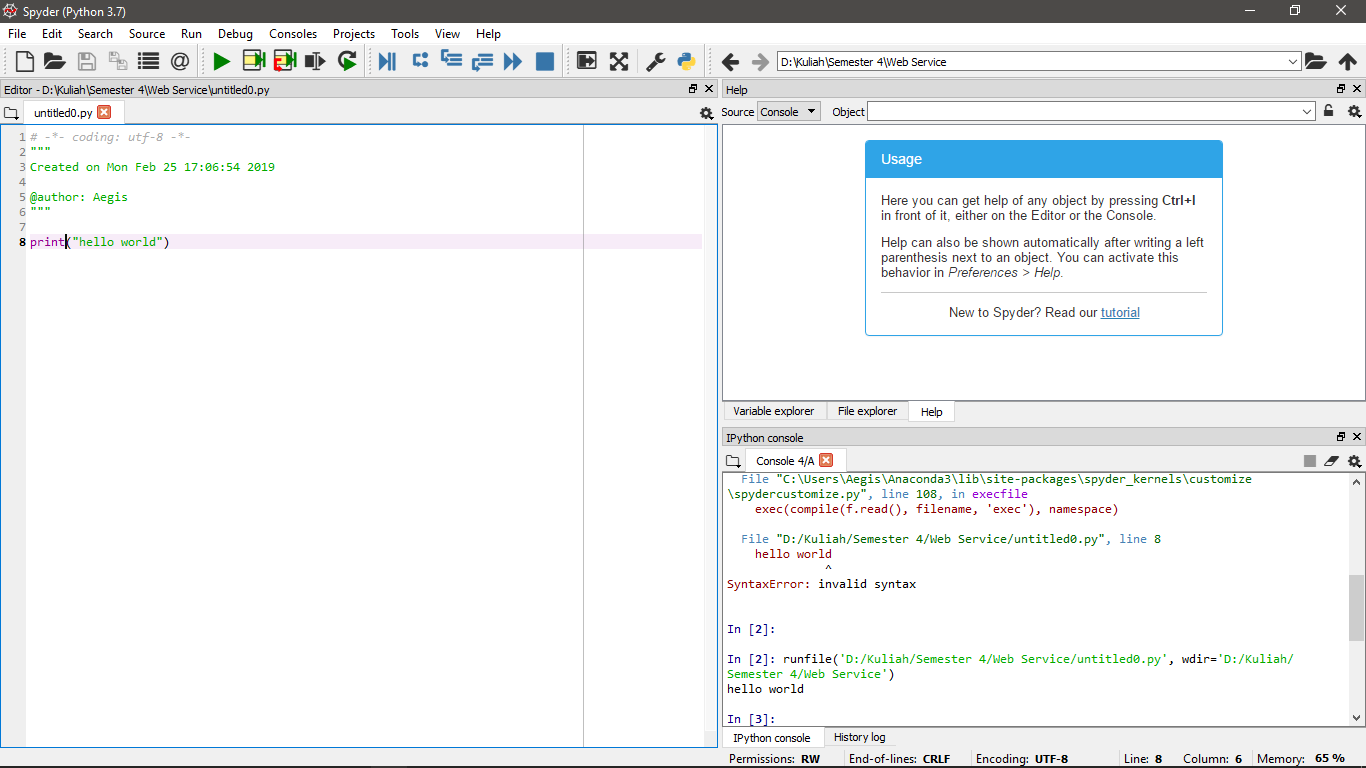
\includegraphics[width=3cm,height=3cm]{figures/Spyder.png}
    \caption{Ini adalah tampilan spyder}
    \label{spyder}
    \end{figure}

Gambar diatas menjelaskan tentang tampilan spider dan mengexsekusi program halo world.

\chapter{Judul Bagian Kedua}
\section{Harun Ar - Rasyid}
\subsection{Teori}
\begin{enumerate}
    \item sebutkan jenis-jenis variabel dan jelaskan cara pemakaian variabel tersebut di
    kode Python
    Variabel merupakan tempat menyimpan data. Dalam phyton kita dapat membuat variable dengan cara sebagai berikut
    \lstinputlisting[firstline=74, lastline=76]{src/1174027.py}

    \item tuliskan bagaimana kode untuk meminta input dari user dan tuliskan bagaimana
    melakukan output ke layar.
    \lstinputlisting[firstline=78, lastline=79]{src/1174027.py}

    \item Tuliskan operator dasar aritmatika, tambah, kali, kurang bagi, dan bagaimana
    mengubah string ke integer dan integer ke string
    Operator  aritmatika adalah operator yang digunakan untuk melakukan perhitungan
    \lstinputlisting[firstline=81, lastline=90]{src/1174027.py}

    \item Tuliskan dan jelaskan sintak untuk perulangan, jenis-jenisnya contoh kode dan
    cara pakainya di python
    Untuk Perulangan Pada Python ada For dan While, Untuk Contohnya bisa lihat gambar berikut :
    \lstinputlisting[firstline=92, lastline=98]{src/1174027.py}

    \item Tuliskan jelaskan cara pakai sintak untuk memilih kondisi, dan bagiamana con-
    toh sintak kondisi di dalam kondisi.
    Pengambilan kondisi If yang digunakan untuk mengantisipasi kondisi yang terjadi saat program dijalankan dan menentukan tindakan apa yang akan diambil sesuai dengan kondisi.
    If statement
    \lstinputlisting[firstline=100, lastline=102]{src/1174027.py}
    
    Ifelse
    \lstinputlisting[firstline=104, lastline=107]{src/1174027.py}
    
    IfNested
    \lstinputlisting[firstline=109, lastline=114]{src/1174027.py}

    \item Tuliskan apa saja jenis error yang sering ditemui di python dalam mengerjakan
    sintak diatas. dan bagaimana cara mengatasinya
    \begin{itemize}
        \item Exception
        Kelas dasar untuk semua pengecualian / exception

        \item Stoplteration
        Dibesarkan ketika metode (iterator) berikutnya dari iterator tidak mengarah ke objek apa pun.

        \item SystemExit
        Dibesarkan oleh fungsi sys.exit ().

        \item StandardError
        Kelas dasar untuk semua pengecualian built-in kecuali StopIteration dan SystemExit.

        \item ArithmeticError
        Kelas dasar untuk semua kesalahan yang terjadi untuk perhitungan numerik.

        \item OverflowError
        Dibesarkan saat perhitungan melebihi batas maksimum untuk tipe numerik.

        \item FloatingPointError
        Dibesarkan saat perhitungan floating point gagal.

        \item ZeroDivisonError
        Dibesarkan saat pembagian atau modulo nol dilakukan untuk semua tipe numerik.

        \item AssertionError
        Dibesarkan jika terjadi kegagalan pernyataan Assert.

        \item AttributeError
        Dibesarkan jika terjadi kegagalan referensi atribut atau penugasan.
         
        \item EOFError
        Dibesarkan bila tidak ada input dari fungsi rawinput () atau input () dan akhir file tercapai.

        \item ImportError
        Dibesarkan saat sebuah pernyataan impor gagal.

        \item KeyboardInterrupt
        Dibesarkan saat pengguna menyela eksekusi program, biasanya dengan menekan Ctrl + c.

        \item LookupError
        Kelas dasar untuk semua kesalahan pencarian.

        \item IndexError
        Dibesarkan saat sebuah indeks tidak ditemukan secara berurutan.

        \item KeyError
        Dibesarkan saat kunci yang ditentukan tidak ditemukan dalam kamus.

        \item NameError
        Dibesarkan saat pengenal tidak ditemukan di namespace lokal atau global.

        \item UnboundLocalError
        Dibesarkan saat mencoba mengakses variabel lokal dalam suatu fungsi atau metode namun tidak ada nilai yang ditugaskan padanya.

        \item EnvironmentError
        Kelas dasar untuk semua pengecualian yang terjadi di luar lingkungan Python.

        \item IOError
        Dibesarkan saat operasi input / output gagal, seperti pernyataan cetak atau fungsi open () saat mencoba membuka file yang tidak ada.

        \item OSError
        Dibangkitkan untuk kesalahan terkait sistem operasi.

        \item SyntaxError
        Dibesarkan saat ada kesalahan dengan sintaks Python.

        \item IndentationError
        Dibesarkan saat indentasi tidak ditentukan dengan benar.

        \item SystemError
        Dibesarkan saat penafsir menemukan masalah internal, namun bila kesalahan ini ditemui juru bahasa Python tidak keluar.

        \item SystemExit
        Dibesarkan saat juru bahasa Python berhenti dengan menggunakan fungsi sys.exit (). Jika tidak ditangani dalam kode, menyebabkan penafsir untuk keluar.

        \item TypeError
        Dibesarkan saat operasi atau fungsi dicoba yang tidak valid untuk tipe data yang ditentukan.

        \item ValueError
        Dibesarkan ketika fungsi bawaan untuk tipe data memiliki jenis argumen yang valid, namun argumen tersebut memiliki nilai yang tidak valid yang ditentukan.

        \item RuntimeError
        Dibesarkan saat kesalahan yang dihasilkan tidak termasuk dalam kategori apa pun.

        \item NotImplementedError
        Dibesarkan ketika metode abstrak yang perlu diimplementasikan di kelas warisan sebenarnya tidak dilaksanakan.
    \end{itemize}

    \item Tuliskan dan jelaskan cara memakai Try Except.
    \lstinputlisting[firstline=116, lastline=122]{src/1174027.py}

\end{enumerate}
\subsection{Ketrampilan Pemrograman}
\begin{enumerate}
    \item Buatlah luaran huruf yang dirangkai dari tanda bintang, pagar atau plus dari
    NPM kita. Tanda bintang untuk NPM mod 3=0, tanda pagar untuk NPM mod
    3 =1, tanda plus untuk NPM mod3=2.
    \lstinputlisting[firstline=7, lastline=17]{src/1174027.py}

    \item Buatlah program hello word dengan input NPM yang disimpan dalam sebuah
    variabel string bernama NPM dan output sebanyak dua dijit belakang NPM.
    \lstinputlisting[firstline=19, lastline=24]{src/1174027.py}
    
    \item Buatlah program hello word dengan input nama yang disimpan dalam sebuah
    variabel string bernama NPM dan beri luaran output berupa tiga karakter
    belakang dari NPM sebanyak penjumlahan tiga dijit tersebut.
    \lstinputlisting[firstline=26, lastline=31]{src/1174027.py}

    \item Buatlah program hello word dengan input nama yang disimpan dalam sebuah
    variabel string bernama NPM dan beri luaran output berupa digit ketiga dari
    belakang dari variabel NPM,
    \lstinputlisting[firstline=33, lastline=35]{src/1174027.py}

    \item Buat program dengan mengisi variabel alfabet
    dengan nomor npm satu persatu berurut.
    \lstinputlisting[firstline=37, lastline=48]{src/1174027.py}

    \item Dari soal no 5, Lakukan penjumlahan dari seluruh variabel tersebut.
    \lstinputlisting[firstline=50, lastline=51]{src/1174027.py}

    \item Dari soal no 5, Lakukan perkalian dari seluruh variabel tersebut.
    \lstinputlisting[firstline=53, lastline=54]{src/1174027.py}

    \item Dari soal no 5, Lakukan print secara vertikal dari NPM anda menggunakan
    variabel diatas.
    \lstinputlisting[firstline=56, lastline=63]{src/1174027.py}

    \item Dari soal no 5, Lakukan print NPM anda tapi hanya dijit genap saja.
    \lstinputlisting[firstline=65, lastline=66]{src/1174027.py}

    \item Dari soal no 5, Lakukan print NPM anda tapi hanya dijit ganjil saja.
    \lstinputlisting[firstline=68, lastline=69]{src/1174027.py}

    \item Dari soal no 5, Lakukan print NPM anda tapi hanya dijit yang termasuk bilan-
    gan prima saja.
    \lstinputlisting[firstline=71, lastline=72]{src/1174027.py}

\end{enumerate}
\subsection{Ketrampilan Penanganan Error}
    \lstinputlisting[language=Python]{src/err2.py}
%%%%%%%%%%%%%%%%%%%%%%%%%%%%%%%%%%%%%%%%%%%%%%%%%%%%%%%%%%%%%%%%%%%%%%%%%%%%%%%%%%%%%%%%%%%%%%%%%%%%%%%%5
\section{Dwi Yulianingsih}
\subsection{Teori}
\begin{enumerate}
    \item Jenis-jenis variable phyton dan cara pemakaiannya
Variabel merupakan tempat menyimpan data. Dalam Phyton terdapat variabel biasa dan variabel array dengan berbagai type data diantaranya adalah variabel dengan type data number, string, dan boolean. Dalam phyton kita dapat membuat variable dengan cara sebagai gambar1 berikut
    \lstinputlisting[firstline=8, lastline=45]{src/teori.py}

    \item Kode untuk meminta input dari user dan bagaimana melakukan output ke layar seperti pada gambar2
    \lstinputlisting[firstline=47, lastline=49]{src/teori.py}

    \item Operator dasar aritmatika
Ada operator penambahan, pengurangan perkalian, perkalian, pembagian, modulus, perpangkatan, dan pembulatan decimal.
    \lstinputlisting[firstline=51, lastline=74]{src/teori.py}

    \item Perulangan
Terdapat dua jenis perulangan di dalam phyton yaitu perulangan while dan perulangan for
    \lstinputlisting[firstline=76, lastline=86]{src/teori.py}

    \item sintak Untuk memilih kondisi, dan kondisi didalam kondisi
Pengambilan kondisi If yang digunakan untuk mengantisipasi kondisi yang terjadi saat program dijalankan dan menentukan tindakan apa yang akan diambil sesuai dengan kondisi.
    \lstinputlisting[firstline=88, lastline=111]{src/teori.py}


    \item Jenis-jenis error pada phyton
Syntax Errors adalah keadaan dimana kode python mengalami kesalahan penulisan. 
ZeroDivisonError adalah eror yang terjadi saat eksekusi program menghasilkan perhitungan matematika pembagian dengan angka nol.
NameError adalah eror yang terjadi saat kode di eksekusi terhadap local name atau global name yang tidak terdefinisi. 
TypeError adalah eror yang terjadi saat dilakukan eksekusi pada suatu operasi atau fungsi dengan type object yang tidak sesuai.

    \item Cara memakai try except
Cara pemakaian try except adalah sebagai berikut :
    \lstinputlisting[firstline=113, lastline=117]{src/teori.py}


\end{enumerate}

\subsection{praktek}
\begin{enumerate}
    \item Jawaban soal no 1
    \lstinputlisting[firstline=7, lastline=17]{src/1174009.py}
    \item Jawaban soal no 2
    \lstinputlisting[firstline=19, lastline=24]{src/1174009.py}
    \item Jawaban soal no 3
    \lstinputlisting[firstline=26, lastline=31]{src/1174009.py}
    \item Jawaban soal no 4
    \lstinputlisting[firstline=33, lastline=35]{src/1174009.py}
    \item Jawaban soal no 5
    \lstinputlisting[firstline=37, lastline=48]{src/1174009.py}
    \item Jawaban soal no 6
    \lstinputlisting[firstline=50, lastline=51]{src/1174009.py}
    \item Jawaban soal no 7
    \lstinputlisting[firstline=53, lastline=54]{src/1174009.py}
    \item Jawaban soal no 8
    \lstinputlisting[firstline=56, lastline=63]{src/1174009.py}
    \item Jawaban soal no 9
    \lstinputlisting[firstline=65, lastline=66]{src/1174009.py}
    \item Jawaban soal no 10
    \lstinputlisting[firstline=68, lastline=69]{src/1174009.py}
    \item Jawaban soal no 11
    \lstinputlisting[firstline=71, lastline=72]{src/1174009.py}
\end{enumerate}

\subsection{Keterampilan dan penanganan eror}
    \lstinputlisting[firstline=8, lastline=15]{src/eror.py}

%%%%%%%%%%%%%%%%%%%%%%%%%%%%%%%%%%%%%%%%%%%%%%%%%%%%%%%%%%

\section{Kadek Diva Krishna Murti}

\subsection{Teori}

\begin{enumerate}
\item Jenis-jenis variabel dan cara pemakaiannya di Python.

\begin{enumerate}
\item Boolean
\lstinputlisting[caption=Contoh kode penggunaan Boolean., firstline=1, lastline=3]{src/1174006.py}

\item String
\lstinputlisting[caption=Contoh kode penggunaan String., firstline=5, lastline=7]{src/1174006.py}

\item Integer
\lstinputlisting[caption=Contoh kode penggunaan Integer., firstline=9, lastline=11]{src/1174006.py}

\item Float
\lstinputlisting[caption=Contoh kode penggunaan Float., firstline=13, lastline=15]{src/1174006.py}

\item Hexadecimal
\lstinputlisting[caption=Contoh kode penggunaan Hexadecimal., firstline=17, lastline=19]{src/1174006.py}

\item Complex
\lstinputlisting[caption=Contoh kode penggunaan Complex., firstline=21, lastline=23]{src/1174006.py}

\item List
\lstinputlisting[caption=Contoh kode penggunaan List., firstline=25, lastline=28]{src/1174006.py}

\item Tuple
\lstinputlisting[caption=Contoh kode penggunaan Tuple., firstline=30, lastline=33]{src/1174006.py}

\item Set
\lstinputlisting[caption=Contoh kode penggunaan Set., firstline=35, lastline=37]{src/1174006.py}

\item Dictionary
\lstinputlisting[caption=Contoh kode penggunaan Dictionary., firstline=40, lastline=43]{src/1174006.py}

\end{enumerate}

\item Kode untuk meminta input dan melakukan output di Python.
\lstinputlisting[caption=Contoh kode input dan output., firstline=45, lastline=48]{src/1174006.py}

\item Operator dasar aritmatika dan mengubah tipe data di Python.

Operator dasar aritmatika
\begin{enumerate}
\item Pertambahan
Operator ini dipergunakan untuk melakukan operasi pertambahan.
\lstinputlisting[caption=Contoh kode operasi pertambahan., firstline=51, lastline=55]{src/1174006.py}
\item Pengurangan
Operator ini dipergunakan untuk melakukan operasi pengurangan.
\lstinputlisting[caption=Contoh kode operasi pengurangan., firstline=57, lastline=61]{src/1174006.py}
\item Perkalian
Operator ini dipergunakan untuk melakukan operasi perkalian.
\lstinputlisting[caption=Contoh kode operasi perkalian., firstline=63, lastline=67]{src/1174006.py}
\item Pembagian
Operator ini dipergunakan untuk melakukan operasi pembagian.
\lstinputlisting[caption=Contoh kode operasi pembagian., firstline=69, lastline=73]{src/1174006.py}
\item Modulus
Operator ini dipergunakan untuk melakukan operasi modulus.
\lstinputlisting[caption=Contoh kode operasi modulus., firstline=75, lastline=79]{src/1174006.py}
\item Perpangkatan
Operator ini dipergunakan untuk melakukan operasi perpangkatan.
\lstinputlisting[caption=Contoh kode operasi perpangkatan., firstline=81, lastline=85]{src/1174006.py}
\item Pembulatan Hasil Bagi
Operator ini dipergunakan untuk melakukan operasi pembulatan hasil bagi.
\lstinputlisting[caption=Contoh kode operasi pembulatan hasil bagi., firstline=87, lastline=91]{src/1174006.py}
\end{enumerate}

Mengubah tipe data
\begin{enumerate}
\item String ke Integer
\lstinputlisting[caption=Contoh kode konversi string ke integer., firstline=94, lastline=97]{src/1174006.py}
\item Integer ke String
\lstinputlisting[caption=Contoh kode konversi integer ke string., firstline=100, lastline=102]{src/1174006.py}
\end{enumerate}


\item Sintak perulangan, jenis-jenisnya, dan cara penggunaannya di Python.
\begin{enumerate}
\item While Loop
While Loop adalah perulangan yang mengeksekusi statement berkali-kali selama kondisi bernilai benar atau True.
\lstinputlisting[caption=Contoh kode penggunaan while loop., firstline=104, lastline=108]{src/1174006.py}

\item For Loop
For Loop  adalah perualangan yang mengulangi item dari urutan apapun, seperti list atau string.
\lstinputlisting[caption=Contoh kode penggunaan for loop., firstline=110, lastline=113]{src/1174006.py}

\item Nested Loop
Nested Loop merupakan perulangan yang berada di perulangan atau biasa disebut dengan perulangan bersarang.
\lstinputlisting[caption=Contoh kode penggunaan nested loop., firstline=115, lastline=122]{src/1174006.py}

\end{enumerate}

\item Sintak pengkodisian dan contoh penggunaannya kondisi di dalam kondisi di Python.
\begin{enumerate}
\item If
Kondisi ini dipergunakan jika penkondisiannya hanya satu.
\lstinputlisting[caption=Contoh kode penggunaan if., firstline=124, lastline=127]{src/1174006.py}

\item If Else
Kondisi ini dipergunakan jika pengkondisiannya ada dua.
\lstinputlisting[caption=Contoh kode penggunaan if else., firstline=129, lastline=134]{src/1174006.py}

\item Elif
Kondisi ini dipergunakan jika pengkondisiannya lebih dari dua.
\lstinputlisting[caption=Contoh kode penggunaan elif., firstline=136, lastline=143]{src/1174006.py}

\item Kondisi di dalam kondisi
Kondisi ini dipergunakan jika pengkondisiannya memerlukan pengkondisian di dalamnya.
\lstinputlisting[caption=Contoh kode penggunaan kondisi di dalam kondisi., firstline=146, lastline=156]{src/1174006.py}

\end{enumerate}

\item Jenis-jenis error dan cara mengatasinya di Python.
\begin{itemize}
\item Syntax Errors
Syntax Errors adalah suatu keadaan saat kode python mengalami kesalahan penulisan. Solusinya adalah memperbaiki penulisan kode yang salah.

\item Zero Division Error
ZeroDivisonError adalah exceptions yang terjadi saat eksekusi program menghasilkan perhitungan matematika pembagian dengan angka nol (0). Solusinya adalah tidak membagi suatu yang hasilnya nol.

\item Name Error
NameError adalah exception yang terjadi saat kode melakukan eksekusi terhadap local name atau global name yang tidak terdefinisi. Solusinya adalah memastikan variabel atau function yang dipanggil ada atau tidak salah ketik.

\item Type Error
TypeError adalah exception yang terjadi saat dilakukan eksekusi terhadap suatu operasi atau fungsi dengan type object yang tidak sesuai. Solusinya adalah mengkoversi varibelnya sesuai dengan tipe data yang akan digunakan.

\end{itemize}

\item Cara pemakaian Try Except di Python.
Berikut ini adalah contoh penggunaan try except.
\lstinputlisting[caption=Contoh kode penggunaan try except., firstline=158, lastline=164]{src/1174006.py}

\end{enumerate}
\hfill \break

\subsection{Ketrampilan Pemrograman}

\begin{enumerate}
\item Jawaban Soal 1
\lstinputlisting[firstline=166, lastline=176]{src/1174006.py}

\item Jawaban Soal 2
\lstinputlisting[firstline=178, lastline=184]{src/1174006.py}

\item Jawaban Soal 3
\lstinputlisting[firstline=186, lastline=192]{src/1174006.py}

\item Jawaban Soal 4
\lstinputlisting[firstline=194, lastline=197]{src/1174006.py}

\item Jawaban Soal 5
\lstinputlisting[firstline=199, lastline=212]{src/1174006.py}

\item Jawaban Soal 6
\lstinputlisting[firstline=215, lastline=217]{src/1174006.py}

\item Jawaban Soal 7
\lstinputlisting[firstline=219, lastline=221]{src/1174006.py}

\item Jawaban Soal 8
\lstinputlisting[firstline=223, lastline=226]{src/1174006.py}

\item Jawaban Soal 9
\lstinputlisting[firstline=228, lastline=233]{src/1174006.py}

\item Jawaban Soal 10
\lstinputlisting[firstline=236, lastline=240]{src/1174006.py}

\item Jawaban Soal 11
\lstinputlisting[firstline=243, lastline=245]{src/1174006.py}

\end{enumerate}
\hfill \break

\subsection{Ketrampilan Penanganan Error}
\begin{enumerate}
\item Jawaban Soal No. 1
\begin{itemize}
\item Syntax Errors
Syntax Errors adalah suatu keadaan saat kode python mengalami kesalahan penulisan. Solusinya adalah memperbaiki penulisan kode yang salah.

\item Zero Division Error
ZeroDivisonError adalah exceptions yang terjadi saat eksekusi program menghasilkan perhitungan matematika pembagian dengan angka nol (0). Solusinya adalah tidak membagi suatu yang hasilnya nol.

\item Name Error
NameError adalah exception yang terjadi saat kode melakukan eksekusi terhadap local name atau global name yang tidak terdefinisi. Solusinya adalah memastikan variabel atau function yang dipanggil ada atau tidak salah ketik.

\item Type Error
TypeError adalah exception yang terjadi saat dilakukan eksekusi terhadap suatu operasi atau fungsi dengan type object yang tidak sesuai. Solusinya adalah mengkoversi varibelnya sesuai dengan tipe data yang akan digunakan.

\end{itemize}

\item Jawaban Soal No. 2																			
\lstinputlisting[firstline=1, lastline=7]{src/2err_1174006.py}
\end{enumerate}
 
 %%%%%%%%%%%%%%%%%%%%%%%%%%%%%%%%%%%%%%%%%%%%%%%%%%%%%%%%%%%%%%%%
 \section{Dezha Aidil Martha}
\subsection{Teori}
\begin{enumerate}
	\item Jenis-jenis variable phyton dan cara pemakaiannya
Variabel merupakan tempat menyimpan data. Dalam Phyton terdapat beberapa variabel dengan berbagai type data diantaranya adalah variabel dengan type data number, string, dan boolean. Dalam phyton kita dapat membuat variable dengan cara sebagai gambar berikut
   \lstinputlisting[firstline=8, lastline=12]{src/1174025_teori.py}
	\item Kode untuk meminta input dari user dan bagaimana melakukan output ke layar
 \lstinputlisting[firstline=67, lastline=68]{src/1174025_teori.py}
	\item Operator dasar aritmatika
Ada operator penambahan, pengurangan perkalian, perkalian, pembagian, modulus, perpangkatan, dan pembulatan decimal.
\lstinputlisting[firstline=71, lastline=94]{src/1174025_teori.py}
	\item Perulangan
Terdapat dua jenis perulangan di dalam phyton yaitu perulangan while dan perulangan for
 \lstinputlisting[firstline=97, lastline=99]{src/1174025_teori.py}
 \lstinputlisting[firstline=102, lastline=105]{src/1174025_teori.py}
	\item sintak Untuk memilih kondisi, dan kondisi didalam kondisi
Pengambilan kondisi If yang digunakan untuk mengantisipasi kondisi yang terjadi saat program dijalankan dan menentukan tindakan apa yang akan diambil sesuai dengan kondisi.
  \lstinputlisting[firstline=108, lastline=111]{src/1174025_teori.py}
  \lstinputlisting[firstline=114, lastline=119]{src/1174025_teori.py}
  \lstinputlisting[firstline=122, lastline=129]{src/1174025_teori.py}

	\item Jenis-jenis error pada phyton
Syntax Errors adalah keadaan dimana kode python mengalami kesalahan penulisan. 
ZeroDivisonError adalah eror yang terjadi saat eksekusi program menghasilkan perhitungan matematika pembagian dengan angka nol.
NameError adalah eror yang terjadi saat kode di eksekusi terhadap local name atau global name yang tidak terdefinisi. 
TypeError adalah eror yang terjadi saat dilakukan eksekusi pada suatu operasi atau fungsi dengan type object yang tidak sesuai.

	\item Cara memakai try except
Cara pemakaian try except adalah sebagai berikut :
\lstinputlisting[firstline=132, lastline=138]{src/1174025_teori.py}

\end{enumerate}

\subsection{praktek}
\begin{enumerate}
	\item Jawaban soal no 1
	\lstinputlisting[firstline=11, lastline=20]{src/1174025_praktek.py}
	\item Jawaban soal no 2
	\lstinputlisting[firstline=24, lastline=28]{src/1174025_praktek.py}
	\item Jawaban soal no 3
	\lstinputlisting[firstline=33, lastline=37]{src/1174025_praktek.py}
	\item Jawaban soal no 4
	\lstinputlisting[firstline=40, lastline=41]{src/1174025_praktek.py}
	\item Jawaban soal no 5
	\lstinputlisting[firstline=44, lastline=56]{src/1174025_praktek.py}
	\item Jawaban soal no 6
	\lstinputlisting[firstline=59, lastline=60]{src/1174025_praktek.py}
	\item Jawaban soal no 7
	\lstinputlisting[firstline=63, lastline=64]{src/1174025_praktek.py}
	\item Jawaban soal no 8
	\lstinputlisting[firstline=67, lastline=71]{src/1174025_praktek.py}
	\item Jawaban soal no 9
	\lstinputlisting[firstline=74, lastline=74]{src/1174025_praktek.py}
	\item Jawaban soal no 10
	\lstinputlisting[firstline=77, lastline=77]{src/1174025_praktek.py}
	\item Jawaban soal no 11
	\lstinputlisting[firstline=80, lastline=80]{src/1174025_praktek.py}
\end{enumerate}

\subsection{Keterampilan dan penanganan eror}
	\lstinputlisting[firstline=10, lastline=17]{src/erro2.py}
%%%%%%%%%%%%%%%%%%%%%%%%%%%%%%%%%%%%%%%%%%%%%%%%%%%%%%%%%%%%%%%%
 \section{Evietania Charis Sujadi}
\subsection{Teori}
\begin{enumerate}
    \item Jenis jenis variable phyton dan cara pemakaiannya
Variabel merupakan tempat menyimpan data. Dalam Phyton terdapat beberapa variabel dengan berbagai type data diantaranya adalah variabel dengan type data number, string, dan boolean. Dalam phyton kita dapat membuat variable dengan cara sebagai gambar berikut
   \lstinputlisting[firstline=8, lastline=12]{src/1174051_teori.py}
    \item Kode untuk meminta input dari user dan bagaimana melakukan output ke layar
 \lstinputlisting[firstline=67, lastline=68]{src/1174051_teori.py}
    \item Operator dasar aritmatika
Ada operator penambahan, pengurangan perkalian, perkalian, pembagian, modulus, perpangkatan, dan pembulatan decimal.
\lstinputlisting[firstline=71, lastline=94]{src/1174051_teori.py}
    \item Perulangan
Terdapat dua jenis perulangan di dalam phyton yaitu perulangan while dan perulangan for
 \lstinputlisting[firstline=97, lastline=99]{src/1174051_teori.py}
 \lstinputlisting[firstline=102, lastline=105]{src/1174051_teori.py}
    \item sintak Untuk memilih kondisi, dan kondisi didalam kondisi
Pengambilan kondisi If yang digunakan untuk mengantisipasi kondisi yang terjadi saat program dijalankan dan menentukan tindakan apa yang akan diambil sesuai dengan kondisi.
  \lstinputlisting[firstline=108, lastline=111]{src/1174051_teori.py}
  \lstinputlisting[firstline=114, lastline=119]{src/1174051_teori.py}
  \lstinputlisting[firstline=122, lastline=129]{src/1174051_teori.py}

    \item Jenis-jenis error pada phyton
Syntax Errors adalah keadaan dimana kode python mengalami kesalahan penulisan. 
ZeroDivisonError adalah eror yang terjadi saat eksekusi program menghasilkan perhitungan matematika pembagian dengan angka nol.
NameError adalah eror yang terjadi saat kode di eksekusi terhadap local name atau global name yang tidak terdefinisi. 
TypeError adalah eror yang terjadi saat dilakukan eksekusi pada suatu operasi atau fungsi dengan type object yang tidak sesuai.

    \item Cara memakai try except
Cara pemakaian try except adalah sebagai berikut :
\lstinputlisting[firstline=132, lastline=138]{src/1174051_teori.py}

\end{enumerate}

\subsection{praktek}
\begin{enumerate}
    \item Jawaban soal no 1
    \lstinputlisting[firstline=11, lastline=20]{src/1174051_praktek.py}
    \item Jawaban soal no 2
    \lstinputlisting[firstline=24, lastline=28]{src/1174051_praktek.py}
    \item Jawaban soal no 3
    \lstinputlisting[firstline=33, lastline=37]{src/1174051_praktek.py}
    \item Jawaban soal no 4
    \lstinputlisting[firstline=40, lastline=41]{src/1174051_praktek.py}
    \item Jawaban soal no 5
    \lstinputlisting[firstline=44, lastline=56]{src/1174051_praktek.py}
    \item Jawaban soal no 6
    \lstinputlisting[firstline=59, lastline=60]{src/1174051_praktek.py}
    \item Jawaban soal no 7
    \lstinputlisting[firstline=63, lastline=64]{src/1174051_praktek.py}
    \item Jawaban soal no 8
    \lstinputlisting[firstline=67, lastline=71]{src/1174051_praktek.py}
    \item Jawaban soal no 9
    \lstinputlisting[firstline=74, lastline=74]{src/1174051_praktek.py}
    \item Jawaban soal no 10
    \lstinputlisting[firstline=77, lastline=77]{src/1174051_praktek.py}
    \item Jawaban soal no 11
    \lstinputlisting[firstline=80, lastline=80]{src/1174051_praktek.py}
\end{enumerate}

\subsection{Keterampilan dan penanganan eror}
    \lstinputlisting[firstline=10, lastline=17]{src/ror.py}
%%%%%%%%%%%%%%%%%%%%%%%%%%%%%%%%%%%%%%%%%%%%%%%%%%%%%%%%%%%%%%%%%%%%%%%%%%%%%%%%%%%%%%%%%%%%%%%%%%%%%%%%%%%%%%
\section{Perintah Navigasi}
Perintah navigasi direktori
\section{Damara Benedikta}
\subsection{Teori}
\begin{enumerate}
	\item jenis-jenis variable phyton dan cara pemakaiannya
Variable merupakan tempat untuk menyimpan data, Isi dari variabel itu dapat berubah atau mutable sesuai dengan operasi yang diinginkan. Saat program dieksekusi maka variabellah yang bertugas menyimpan data. Dimana didalam phyton terdapat beberapa variable diantaranya number, boolean,string. Dalam membuat variabel Pythoncaranya adalah sebagai berikut
    \lstinputlisting[firstline=8,lastline=46]{src/teori1.py}
    \item operator dasar aritmatika 
dimana terdapat penjumlahan,pengurangan,pembagian,perkalian,perpangkatan,pembulatan nominal
    \lstinputlisting[firstline=47,lastline=75]{src/teori1.py}
    \item Perulangan
dalam phyton terdapat perulangan while dan for
    \lstinputlisting[firstline=76,lastline=87]{src/teori1.py}
    \item Dimana terdapat sintak untuk meilih kondisi didalam kondisi
Untuk memilih keputusan menggunakan (kondisi if) dimana digunakan untuk mengantisipasi kondisi yang terjadi saat jalannya suatu program dan menentukan tindakan apa yang akan dilakukan sesuai dengan kondisi.
    \lstinputlisting[firstline=88,lastline=112]{src/teori1.py}

    \item Jenis-jenis sintak error pada phyton
 Syntax errors Jika dalam program terdapat kesalahan sintaks maka proses akan berhenti dan menampilkan pesan kesalahan.
Runtime errors, disebut begitu karenakesalahan tidak akan muncul sampai Anda menjalankan program tersebut.Kesalahan ini juga dikenal dengan exceptions atau pengecualian karena biasanya mengindikasikan sesuatu pengecualian yang buruk telah terjadi.

Type eror merupakan eror yang terjadi saat dilakukan eksekusi pada suatu operasi dengan type object yang tidak sesuai.
ZeroDivision eror merupakan eror yang terjadi saat eksekusi program menghasilkan perhitungan matematika dengan angka 0

 \item Try except
cara memakai try except adalah sebagai berikut
    \lstinputlisting[firstline=8,lastline=17]{src/teori1.py}
    \end{enumerate}
\subsection{praktek}
\begin{enumerate}
	\item Jawaban soal no 1
	\lstinputlisting[firstline=8,lastline=17]{src/1174012.py}
	\item Jawaban soal no 2
	\lstinputlisting[firstline=18,lastline=23]{src/1174012.py}
	\item Jawaban soal no 3
	\lstinputlisting[firstline=24,lastline=29]{src/1174012.py}
	\item Jawaban soal no 4
	\lstinputlisting[firstline=30,lastline=32]{src/1174012.py}
	\item Jawaban soal no 5
	\lstinputlisting[firstline=33,lastline=43]{src/1174012.py}
	\item Jawaban soal no 6
	\lstinputlisting[firstline=44,lastline=45]{src/1174012.py}
	\item Jawaban soal no 7
	\lstinputlisting[firstline=46,lastline=47]{src/1174012.py}
	\item Jawaban soal no 8
	\lstinputlisting[firstline=48,lastline=55]{src/1174012.py}
	\item Jawaban soal no 9
	\lstinputlisting[firstline=56,lastline=57]{src/1174012.py}
	\item Jawaban soal no 10
	\lstinputlisting[firstline=58,lastline=59]{src/1174012.py}
	\item Jawaban soal no 11
	\lstinputlisting[firstline=60,lastline=61]{src/1174012.py}
\end{enumerate}

\subsection{Keterangan dan Penanganan eror}
\lstinputlisting[firstline=5,lastline=15]{src/error1.py}





\bibliographystyle{IEEEtran} 
%\def\bibfont{\normalsize}
\bibliography{references}


%%%%%%%%%%%%%%%
%%  The default LaTeX Index
%%  Don't need to add any commands before \begin{document}
\printindex

%%%% Making an index
%% 
%% 1. Make index entries, don't leave any spaces so that they
%% will be sorted correctly.
%% 
%% \index{term}
%% \index{term!subterm}
%% \index{term!subterm!subsubterm}
%% 
%% 2. Run LaTeX several times to produce <filename>.idx
%% 
%% 3. On command line, type  makeindx <filename> which
%% will produce <filename>.ind 
%% 
%% 4. Type \printindex to make the index appear in your book.
%% 
%% 5. If you would like to edit <filename>.ind 
%% you may do so. See docs.pdf for more information.
%% 
%%%%%%%%%%%%%%%%%%%%%%%%%%%%%%

%%%%%%%%%%%%%% Making Multiple Indices %%%%%%%%%%%%%%%%
%% 1. 
%% \usepackage{multind}
%% \makeindex{book}
%% \makeindex{authors}
%% \begin{document}
%% 
%% 2.
%% % add index terms to your book, ie,
%% \index{book}{A term to go to the topic index}
%% \index{authors}{Put this author in the author index}
%% 
%% \index{book}{Cows}
%% \index{book}{Cows!Jersey}
%% \index{book}{Cows!Jersey!Brown}
%% 
%% \index{author}{Douglas Adams}
%% \index{author}{Boethius}
%% \index{author}{Mark Twain}
%% 
%% 3. On command line type 
%% makeindex topic 
%% makeindex authors
%% 
%% 4.
%% this is a Wiley command to make the indices print:
%% \multiprintindex{book}{Topic index}
%% \multiprintindex{authors}{Author index}

\end{document}

